\documentclass[problems]{esg8022pset} 
  \usepackage{amsmath}
  \usepackage{amssymb}
  \usepackage{enumerate}
  \usepackage{graphicx}
  \usepackage{hyperref}
  %\usepackage{siunitx}
  \providecommand{\uvec}[1]{{\hat{\bf{#1}}}}
  \usepackage{pgf,tikz}
  \usetikzlibrary{arrows}
  \usepackage{wasysym}
  \makeatletter
  \newcommand{\interitemtext}[1]{%
    \begin{list}{}
     {\itemindent=0mm\labelsep=0mm
     \labelwidth=0mm\leftmargin=0mm
     \addtolength{\leftmargin}{-\@totalleftmargin}}
      \item #1
    \end{list}
  }
  \makeatother
  \renewcommand{\d}{\,d}
  \providecommand{\norm}[1]{\lVert#1\rVert}
\classname{Physics 8.022} \semester{Spring 2011} 
\problemsetnumber{1} 
\date{\today } 
\duedate{Sunday, February 6} 
\readingassignment{} 
\psettitle{Systems of charges and electric fields} 
\begin{document}
\section{Problem \thesection: Purcell 1.3}
  Two volley balls, mass 0.3 kilogram (kg) each, tethered by nylon strings and charged with an electrostatic generator, hang as shown in the diagram. What is the charge on each in coulombs, assuming the charges are equal? (\emph{Reminder}: the weight of a 1-kg mass on earth is 9.8 newtons, just as the weight of a 1-gm mass is 980 dynes.)
  \begin{center}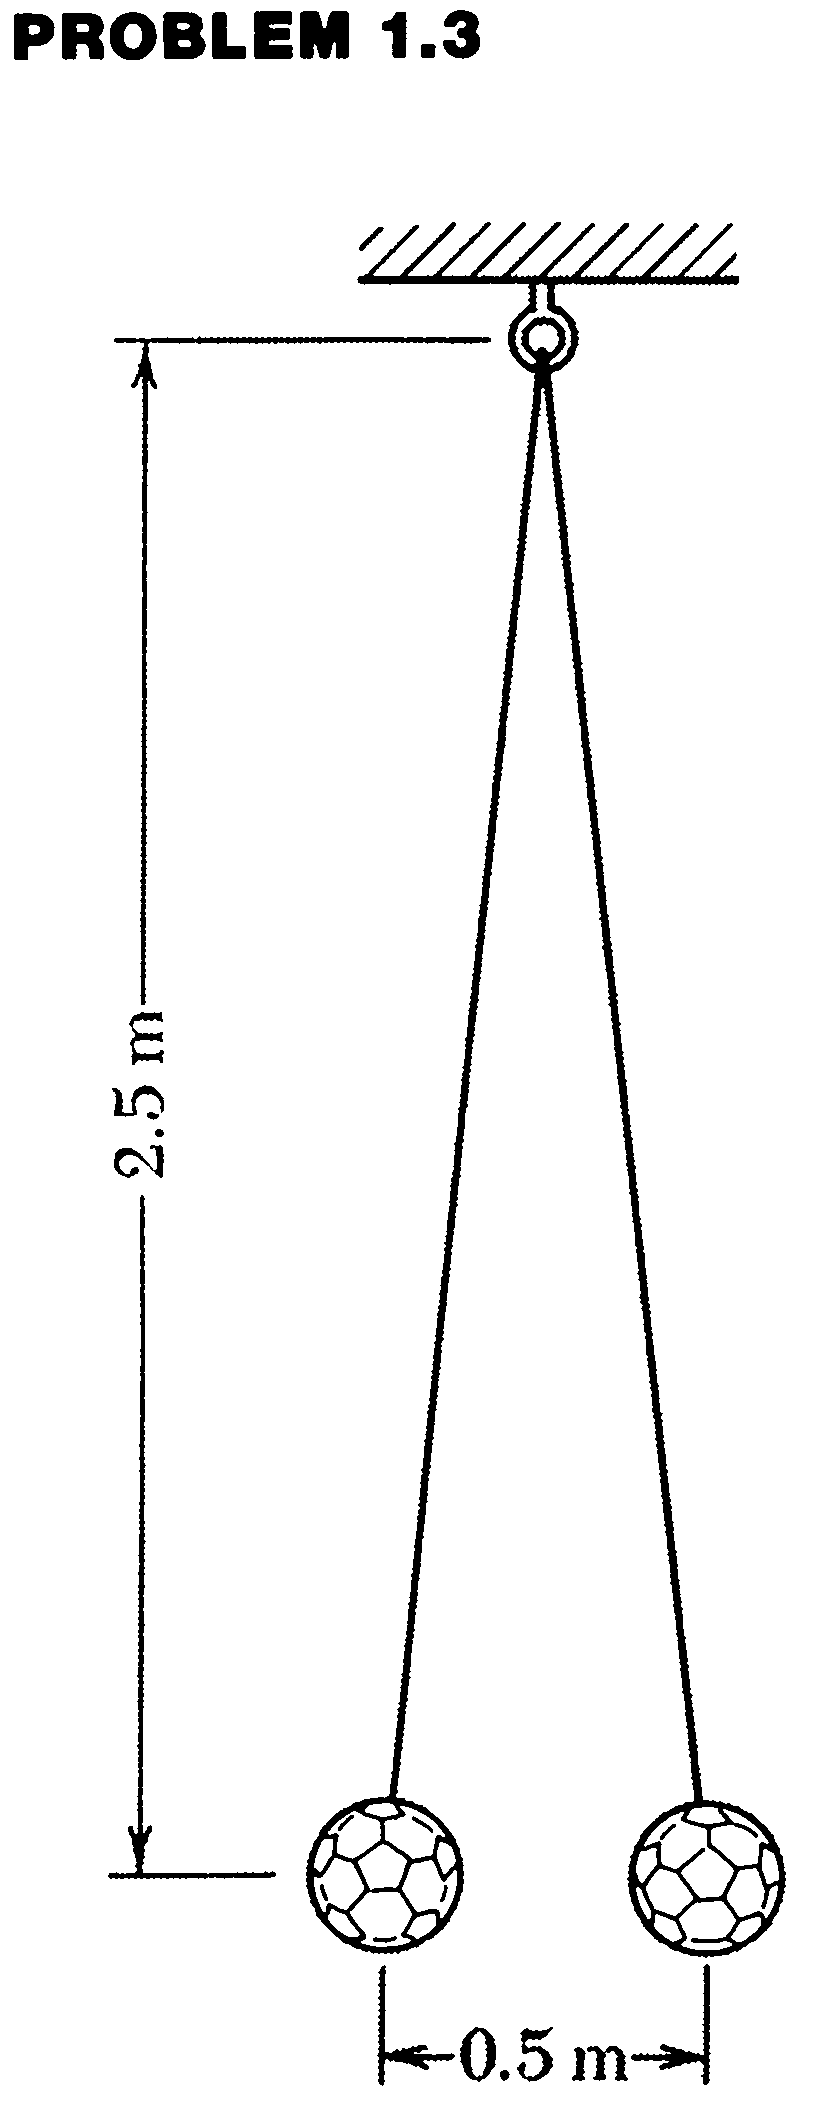
\includegraphics[width=0.2\textwidth]{ps01_1}\end{center}
\section{Problem \thesection: Purcell 1.5}
  A thin plastic rod bent into a semicircle of radius $R$ has a charge of $Q$, in esu, distributed uniformly over its length. Find the strength of the electric field at the center of the semicircle.
\section{Problem \thesection: Purcell 1.8}
  Calculate the potential energy, per ion, for an infinite one-dimensional ionic crystal, that is, a row of equally spaced charges of magnitude $e$ and alternating sign.

  \noindent [\emph{Hint}: The power series expansion of $\ln(1+x)$,
  $$\ln(1+x) = \sum_{j=1}^\infty \frac{(-x)^{j-1}}{j},$$
  may be of use.]
\section{Problem \thesection: Purcell 1.9 (next week we will solve the same problem in a different way)}
  A spherical volume of radius $a$ is filled with charge of uniform density $\rho$. We want to know the potential energy $U$ of this sphere of charge, that is, the work done in assembling it. Calculate it by building the sphere up layer by layer.  Express the result in terms of the total charge $Q$ in the sphere.
  \begin{flushright}\emph{Ans}. $U = \frac35 (Q^2 / a)$\end{flushright}
\section{Problem \thesection: Purcell 1.11}
  A charge of 1 esu is at the origin. A charge of $-2$ esu is at $x = 1$ on the $x$ axis.
  \begin{enumerate}[(a)]
    \item Find a point on the $x$ axis where the electric field is zero.
    \item Locate, at least approximately, a point on the $y$ axis where the electric field is parallel to the $x$ axis.
  \end{enumerate}
\section{Problem \thesection: Purcell 1.12}
  Two positive ions and one negative ion are fixed at the vertices of an equilateral triangle.  Where can a fourth ion be placed so that the force on it will be zero?  Is there more than one such place?

  Note, the ions all have the same \emph{magnitude} of charge, i.e., the charges are $+Q$, $+Q$, and $-Q$. You may consider only solutions that lie on the axis of symmetry. Are there other possible solutions?

  \textsc{Optional}: Use Mathematica (\url{http://ist.mit.edu/services/software/mathematica/obtain}) or Wolfram Alpha (\url{http://www.wolframalpha.com/}) to solve the final equation.
\section{Problem \thesection: Electric Dipole}
  A pair of charges lie in the $xy$-plane.  The charge $q$ is at coordinate $x = 0$, $y = b$; the charge $-q$ is at coordinate $x = 0$, $y = -b$.
  \begin{center}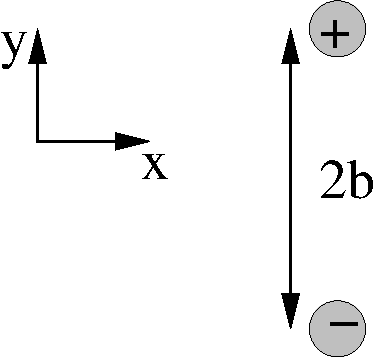
\includegraphics[width=0.2\textwidth]{ps01_8}\end{center}
  \begin{enumerate}[(a)]
    \item Evaluate the electric field (magnitude \emph{and} direction) on the $x$-axis.  Show that for $x \gg b$, $|\vec E| \propto 1 / x^3$.  What is the direction in this limit?
    \item Evaluate the electric field on the $y$-axis.  Consider $y < -b$, $-b < y < b$, and $b < y$ separately.  Additionally, find the magnitude and direction for $y \gg b$.
  \end{enumerate}
\section{Problem \thesection: Coulomb force between line charges}
  A rod of length $l_1$ with linear charge density $\lambda_1$ and a rod of length $l_2$ with linear charge density $\lambda_2$ lie on the $x$-axis.  Their ends are separated by a distance $D$ as shown in the figure.
  \begin{center}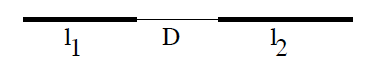
\includegraphics[width=0.4\textwidth]{ps01_9}\end{center}
  Assume that the charge densities have the same sign.
  \begin{enumerate}[(a)]
    \item What is the force $\vec F$ between these charges?
    \item Show that for $D \gg l_1$ and $D \gg l_2$, this force reduces to the Coulomb forces between a pair of point charges, $q_1 = l_1\lambda_1$, $q_2 = l_2\lambda_2$.
  \end{enumerate}
\end{document}
